%Fred, Mac, Yuhan NSF Grant Dec 2019
% GitHub: https://github.com/fjhickernell/NSF_CompMath2018Nov
% Overleaf: https://www.overleaf.com/9576964687whkhbmrrvhsd
\documentclass[11pt]{NSFamsart}
\usepackage{latexsym,amsfonts,amsmath,amssymb,amsthm,epsfig,extdash,multirow}
\usepackage{stackrel,tabularx,mathtools,enumitem,longtable,xspace}
\usepackage[dvipsnames]{xcolor}
\usepackage[numbers,sort&compress]{natbib}
\usepackage{hyperref,accents, booktabs}
\usepackage{algorithm, algorithmicx}
\usepackage{anyfontsize}
\usepackage{cleveref}
\usepackage{wrapfig}
%\usepackage[letterpaper,total={6in, 9in},top  = 1in, bmargin = 1in]{geometry}
\usepackage[font=small,labelfont=bf]{caption}
%\usepackage[sort&compress]{natbib}

\voffset 0.1in
\textheight 8.8 in
\pagestyle{empty}
\thispagestyle{empty}

\usepackage{algpseudocode}
\algnewcommand\algorithmicparam{\textbf{Parameters:}}
\algnewcommand\PARAM{\item[\algorithmicparam]}
\algnewcommand\algorithmicinput{\textbf{Input:}}
\algnewcommand\INPUT{\item[\algorithmicinput]}
%\algnewcommand\STATE{\item}
\algnewcommand\RETURN{\State \textbf{Return }}

%\usepackage{showlabels}
\newcommand{\Upara}[1]{\noindent\underline{\upshape #1}:}

\newcommand{\myshade}{60}
\colorlet{mylinkcolor}{violet}
\colorlet{mycitecolor}{violet}
%\colorlet{mycitecolor}{OliveGreen}
\colorlet{myurlcolor}{YellowOrange}

\hypersetup{
	linkcolor  = mylinkcolor!\myshade!black,
	citecolor  = mycitecolor!\myshade!black,
	urlcolor   = myurlcolor!\myshade!black,
	colorlinks = true,
}


% This package prints the labels in the margin
%\usepackage[notref,notcite]{showkeys}

%\numberwithin{page} %add section before page
\pagestyle{plain}
%\setcounter{page}{1}
%\renewcommand{\thepage}{C-\arabic{page}}

%\thispagestyle{empty} \pagestyle{empty} %to eliminate page numbers for upload
%\thispagestyle{plain} \pagestyle{plain} %to add back page numbers

\headsep-0.6in
%\headsep-0.45in

%%list of acronyms with links
\newcommand{\QMCSoft}{QMCSoft\xspace}
\newcommand{\GAIL}{GAIL\xspace}
\newcommand{\QMC}{QMC\xspace}
\newcommand{\IIDMC}{IID MC\xspace}
\newcommand{\SAMSIQMC}{SAMSI-QMC\xspace}
\newcommand{\SciPy}{SciPy\xspace}
\newcommand{\GSL}{GSL\xspace}
\newcommand{\NAG}{NAG\xspace}
\newcommand{\MATLAB}{MATLAB\xspace}
\newcommand{\Chebfun}{Chebfun\xspace}
\newcommand{\Rlang}{R\xspace}
\newcommand{\Julia}{Julia\xspace}


\textwidth6.5in
\setlength{\oddsidemargin}{0in}
\setlength{\evensidemargin}{0in}
\textheight9.0in
%\textheight9.1in

\newtheorem{theorem}{theorem}


\providecommand{\FJHickernell}{Hickernell}
\newcommand{\hf}{\widehat{f}}
\newcommand{\hg}{\widehat{g}}
\newcommand{\hI}{\hat{I}}
\newcommand{\hatf}{\hat{f}}
\newcommand{\hatg}{\hat{g}}
\newcommand{\tf}{\widetilde{f}}
\newcommand{\tbf}{\tilde{\bff}}
%\DeclareMathOperator{\Pr}{\mathbb{P}}

% Math operators
\DeclareMathOperator{\std}{std}
\DeclareMathOperator{\cost}{COST}
\DeclareMathOperator{\comp}{COMP}
\DeclareMathOperator{\loss}{loss}
\DeclareMathOperator{\lof}{lof}
\DeclareMathOperator{\reg}{reg}
\DeclareMathOperator{\CV}{CV}
\DeclareMathOperator{\size}{wd}
\DeclareMathOperator{\GP}{\mathcal{G} \! \mathcal{P}}
\DeclareMathOperator{\erf}{erf}
\DeclareMathOperator*{\argmax}{arg\,max}
\DeclareMathOperator*{\argmin}{arg\,min}
\DeclareMathOperator{\QOI}{QOI} %Quantity of Interest
\DeclareMathOperator{\POI}{POI} %Parameter of Interest
\DeclareMathOperator{\Ans}{ANS}
\DeclareMathOperator{\Var}{Var}
\DeclareMathOperator{\APP}{\widehat{\QOI}}
\DeclareMathOperator{\SURR}{SM} %surrogate model
\DeclareMathOperator{\STREND}{ST} %surrogate trend
\DeclareMathOperator{\SVAR}{SV} %surrogate variation
\DeclareMathOperator{\SVARERR}{SVU} %surrogate variation uncertainty
\newcommand{\MLS}{\textrm{MLS}\xspace} %distance weighted least squares, also known as moving least squares
%\DeclareMathOperator{\ALG}{ALG}
\DeclareMathOperator{\ERR}{ERR}
\DeclareMathOperator{\VAL}{ACQ}
\DeclareMathOperator{\OPER}{OPER}
\DeclareMathOperator{\INT}{INT}
\DeclareMathOperator{\MIN}{MIN}
\DeclareMathOperator{\ID}{ID}
\DeclareMathOperator{\APPMIN}{\widehat{\MIN}}
\DeclareMathOperator{\APPID}{\widehat{\ID}}
\DeclareMathOperator{\MINVAL}{MINACQ}
\DeclareMathOperator{\IDVAL}{IDACQ}
\DeclareMathOperator{\SURRERR}{SU}
\DeclareMathOperator{\MINERR}{MERR}
\DeclareMathOperator{\IDERR}{IDERR}
\DeclareMathOperator{\Prob}{\mathbb{P}}
\DeclareMathOperator{\diag}{diag}
\DeclareMathOperator{\dist}{dist}
\DeclareMathOperator{\filldis}{fill}
\DeclareMathOperator{\sep}{sep}
\DeclareMathOperator{\avg}{avg}
\DeclareMathOperator{\vol}{vol}
\DeclareMathOperator{\cov}{cov}
\newcommand{\TREND}{\textup{T}}
\newcommand{\VAR}{\textup{V}}
\newcommand{\LS}{\textup{LS}}







\newcommand{\reals}{{\mathbb{R}}}
\newcommand{\naturals}{{\mathbb{N}}}
\newcommand{\natzero}{{\mathbb{N}_0}}
\newcommand{\integers}{{\mathbb{Z}}}
\def\expect{{\mathbb{E}}}
\def\il{\left \langle}
\def\ir{\right \rangle}
\def\e{\varepsilon}
\def\g{\gamma}
\def\l{\lambda}
\def\b{\beta}
\def\a{\alpha}
\def\lall{\Lambda^{{\rm all}}}
\def\lstd{\Lambda^{{\rm std}}}

\newcommand{\vf}{\boldsymbol{f}}
\newcommand{\hV}{\widehat{V}}
\newcommand{\tV}{\widetilde{V}}
\newcommand{\fraku}{\mathfrak{u}}
\newcommand{\hcut}{\mathfrak{h}}
\newcommand{\tOmega}{\widetilde{\Omega}}
\newcommand{\tvarrho}{\widetilde{\varrho}}

\newcommand{\bbE}{\mathbb{E}}
\newcommand{\tQ}{\widetilde{Q}}
\newcommand{\mA}{\mathsf{A}}
\newcommand{\mB}{\mathsf{B}}
\newcommand{\mC}{\mathsf{C}}
\newcommand{\mD}{\mathsf{D}}
\newcommand{\mG}{\mathsf{G}}
\newcommand{\mH}{\mathsf{H}}
\newcommand{\mI}{\mathsf{I}}
\newcommand{\bbK}{\mathbb{K}}
\newcommand{\mK}{\mathsf{K}}
\newcommand{\tmK}{\widetilde{\mathsf{K}}}
\newcommand{\mL}{\mathsf{L}}
\newcommand{\mM}{\mathsf{M}}
\newcommand{\mP}{\mathsf{P}}
\newcommand{\mQ}{\mathsf{Q}}
\newcommand{\mR}{\mathsf{R}}
\newcommand{\mX}{\mathsf{X}}
\newcommand{\mPhi}{\mathsf{\Phi}}
\newcommand{\mPsi}{\mathsf{\Psi}}
\newcommand{\mLambda}{\mathsf{\Lambda}}
\newcommand{\cube}{[0,1]^d}
\newcommand{\design}{\{\bx_i\}_{i=1}^n}




\newcommand{\bone}{\boldsymbol{1}}
\newcommand{\bzero}{\boldsymbol{0}}
\newcommand{\binf}{\boldsymbol{\infty}}
\newcommand{\ba}{{\boldsymbol{a}}}
\newcommand{\bb}{{\boldsymbol{b}}}
\newcommand{\bc}{{\boldsymbol{c}}}
\newcommand{\bd}{{\boldsymbol{d}}}
\newcommand{\be}{{\boldsymbol{e}}}
\newcommand{\bff}{{\boldsymbol{f}}}
\newcommand{\bhh}{{\boldsymbol{h}}}
\newcommand{\beps}{{\boldsymbol{\varepsilon}}}
\newcommand{\tbeps}{\tilde{\beps}}
\newcommand{\bt}{{\boldsymbol{t}}}
\newcommand{\bT}{{\boldsymbol{T}}}
\newcommand{\bx}{{\boldsymbol{x}}}
\newcommand{\bX}{{\boldsymbol{X}}}
\newcommand{\bh}{{\boldsymbol{h}}}
\newcommand{\bj}{{\boldsymbol{j}}}
\newcommand{\bk}{{\boldsymbol{k}}}
\newcommand{\bg}{{\boldsymbol{g}}}
\newcommand{\bn}{{\boldsymbol{n}}}
\newcommand{\br}{{\boldsymbol{r}}}
\newcommand{\bv}{{\boldsymbol{v}}}
\newcommand{\bu}{{\boldsymbol{u}}}
\newcommand{\by}{{\boldsymbol{y}}}
\newcommand{\bz}{{\boldsymbol{z}}}
\newcommand{\bvarphi}{{\boldsymbol{\varphi}}}
\newcommand{\bgamma}{{\boldsymbol{\gamma}}}
\newcommand{\bphi}{{\boldsymbol{\phi}}}
\newcommand{\bpsi}{{\boldsymbol{\psi}}}
\newcommand{\btheta}{{\boldsymbol{\theta}}}
\newcommand{\bnu}{{\boldsymbol{\nu}}}
\newcommand{\balpha}{{\boldsymbol{\alpha}}}
\newcommand{\bbeta}{{\boldsymbol{\beta}}}
\newcommand{\bo}{{\boldsymbol{\omega}}}  %GF added
\newcommand{\newton}[2]{\left(\begin{array}{c} #1\\ #2\end{array}\right)}
\newcommand{\anor}[2]{\| #1\|_{\mu_{#2}}}
\newcommand{\satop}[2]{\stackrel{\scriptstyle{#1}}{\scriptstyle{#2}}}
\newcommand{\setu}{{\mathfrak{u}}}

\newcommand{\me}{\textup{e}}
\newcommand{\mi}{\textup{i}}
\def\d{\textup{d}}
\def\dif{\textup{d}}
\newcommand{\cc}{\mathcal{C}}
\newcommand{\cb}{\mathcal{B}}
\newcommand{\cl}{L}
\newcommand{\ct}{\mathfrak{T}}
\newcommand{\cx}{{\Omega}}
\newcommand{\cala}{{\mathcal{A}}}
\newcommand{\calc}{{\mathcal{C}}}
\newcommand{\calf}{{\mathcal{F}}}
\newcommand{\calfd}{{\calf_d}}
\newcommand{\calh}{{\mathcal{H}}}
\newcommand{\tcalh}{{\widetilde{\calh}}}
\newcommand{\calI}{{\mathcal{I}}}
\newcommand{\calhk}{\calh_d(K)}
\newcommand{\calg}{{\mathcal{G}}}
\newcommand{\calgd}{{\calg_d}}
\newcommand{\caln}{{\mathcal{N}}}
\newcommand{\calp}{{\mathcal{P}}}
\newcommand{\cals}{{\mathcal{S}}}
\newcommand{\calu}{{\mathcal{U}}}
\newcommand{\cL}{\mathcal{L}}
\newcommand{\cP}{\mathcal{P}}
\newcommand{\cT}{\mathcal{T}}
\newcommand{\cK}{\mathcal{K}}
\newcommand{\fA}{\mathfrak{A}}
\newcommand{\fC}{\mathfrak{C}}
\newcommand{\fF}{\mathfrak{F}}
\newcommand{\fL}{\mathfrak{L}}
\newcommand{\fU}{\mathfrak{U}}
\newcommand{\hS}{\widehat{S}}

\def\abs#1{\ensuremath{\left \lvert #1 \right \rvert}}
\newcommand{\bigabs}[1]{\ensuremath{\bigl \lvert #1 \bigr \rvert}}
\newcommand{\norm}[2][{}]{\ensuremath{\left \lVert #2 \right \rVert}_{#1}}
\newcommand{\ip}[3][{}]{\ensuremath{\left \langle #2, #3 \right \rangle_{#1}}}
\newcommand{\bignorm}[2][{}]{\ensuremath{\bigl \lVert #2 \bigr \rVert}_{#1}}
\newcommand{\Bignorm}[2][{}]{\ensuremath{\Bigl \lVert #2 \Bigr \rVert}_{#1}}
\newcommand{\calm}{{\mathfrak{M}}}

\newcommand{\des}{\{\bx_i\}}
\newcommand{\desinf}{\{\bx_i\}_{i=1}^{\infty}}
\newcommand{\desn}{\{\bx_i\}_{i=1}^n}
\newcommand{\wts}{\{g_i\}_{i=1}^N}
\newcommand{\wtsn}{\{g_i\}_{i=1}^N}
\newcommand{\datan}{\{y_i\}_{i=1}^N}

%FJH added
\newcommand{\Order}{\mathcal{O}}
\newcommand{\ch}{\mathcal{H}}
\newcommand{\tch}{{\widetilde{\ch}}}
\newcommand{\veps}{\boldsymbol{\varepsilon}}
\DeclareMathOperator{\best}{best}
\newcommand{\hmu}{\hat{\mu}}
\newcommand{\hsigma}{\hat{\sigma}}
\newcommand{\tK}{\widetilde{K}}
%\newcommand{\Matlab}{{\sc Matlab}\xspace}
\newcommand{\abstol}{\varepsilon_{\text{a}}}
\newcommand{\reltol}{\varepsilon_{\text{r}}}

\newcommand\starred[1]{\accentset{\star}{#1}}

\newcommand{\designInf}{\{\bx_i\}_{i=1}^\infty}
\newcommand{\dataN}{\bigl\{\bigl(\bx_i,f(\bx_i)\bigr)\bigr\}_{i=1}^n}
\newcommand{\dataNp}{\bigl\{\bigl(\bx_i,f(\bx_i)\bigr)\bigr\}_{i=1}^{n'}}
\newcommand{\dataNo}{\bigl\{\bigl(\bx_i,f(\bx_i)\bigr)\bigr\}_{i=1}^{n_0}}
\newcommand{\ErrN}{\ERR\bigl(\dataN,n\bigr)}
\newcommand{\fint}{f_{\text{int}}}
\newcommand{\inflate}{\fC}
\newcommand{\IIDSim}{\overset{\text{IID}}{\sim}}
\newcommand{\LDSim}{\overset{\text{LD}}{\sim}}


\definecolor{MATLABOrange}{rgb}{0.85,  0.325, 0.098}


%\setcounter{page}{1}


\setlist[description]{font=\normalfont\itshape, labelindent = 0.5cm}
\setlist[itemize]{leftmargin=5ex}

\makeatletter
\newenvironment{varsubequations}[1]
 {%
  \addtocounter{equation}{-1}%
  \begin{subequations}
  \renewcommand{\theparentequation}{#1}%
  \def\@currentlabel{#1}%
 }
 {%
  \end{subequations}\ignorespacesafterend
 }
\makeatother


\newcommand{\FJHNote}[1]{{\color{blue}Fred: #1}}
\newcommand{\JMHNote}[1]{{\color{green}Mac: #1}}

% Notes on the paper for communicating with coauthors
\newif\ifnotesw \noteswtrue
\newcommand{\notes}[1]{\ifnotesw \textcolor{red}{  $\clubsuit$\ {\sf \bf \it  #1}\ $\clubsuit$  }\fi}
%\noteswfalse   % comment this line out to turn on style notes 
\begin{document}
%\setlength{\leftmargini}{2.5ex}

\begin{center}
\Large \textbf{
QMCPy: Quasi-Monte Carlo Community Software\\ 
%Project Description
}
\end{center}
\vspace{-2ex}

\setcounter{tocdepth}{1}
\tableofcontents

\vspace{-6ex}

\section{Overview of QMC}

Quasi-Monte Carlo (QMC) methods replace independent and identically distributed (IID) points by low discrepancy (LD) points to achieve substantial efficiency gains.  We propose to grow QMCPy \cite{QMCPy2020a}, a Python QMC software library, which will be embraced by QMC researchers and benefit an expanding base of QMC users.  QMCPy will become
\begin{enumerate}
\renewcommand{\labelenumi}{\arabic{enumi}.}
    \item A structured collection of the best QMC software, including
    \begin{enumerate}
    \renewcommand{\labelenumii}{\alph{enumii}.}
        \item LD sequence generators,
        \item QMC algorithms, such as multi-level algorithms, automatic stopping criteria, and variance/variation reduction, and
        \item Illuminating use cases,
    \end{enumerate}
    \item A user-friendly, consistent interface to the contributions of many,
    \item A proving ground for new QMC ideas,
    \item Owned and cultivated by our QMC community, and
    \item An easy on-ramp for those who are new to QMC.
\end{enumerate}

\subsection{Applications of (Q)MC}  Many situations are best understood by building randomness into the mathematical model.  Examples include statistical inference \cite{}, financial risk \cite{Gla03}, light transport \cite{}, uncertainty quantification \cite{}, and particle physics \cite{}.  Simulations using random vectors or discrete stochastic processes to generate a myriad of possible outcomes.  The statistical properties of these sample outcomes---such as means (averages), quantiles, and probability densities---can effectively estimate the population quantities.  This is the (Q)MC process---IID sampling for simple MC and LD sampling for QMC.

(Q)MC simulation is efficient for computing multivariate integrals since it avoids the curse of dimensionality inherent in tensor product cubature rules.  Cubature based on grid sampling has a cost that increases exponentially with the number of variables.

In construction of surrogate models for computer experiments (multivariate function approximation), one often wishes to evenly sample the domain to search for regions where the function changes more sharply.  IID and LD sampling again proves advantageous over grid sampling.

\subsection{LD Versus IID Sampling}

The quantity of interest, $Y$ (option payoff, pixel intensity, time to failure), is commonly expressed as a function of a $d$-dimensional vector random variable $\bX$, i.e., $Y = f(\bX)$.  We assume that $\bX$ follows a cumulative distribution function $F:\cx \subseteq \reals^d \to [0,1]$.  When $f$ has a complicated form, the population mean (multivariate integral), 
\begin{equation}
    \mu = \bbE(Y) = \int_{\cx} f(\bx) \, \dif F(\bx),
\end{equation} 
cannot be computed analytically but may be estimated the sample mean,
\begin{equation}
\hmu_n = \frac 1n \sum_{i=1}^n Y_i = \frac 1n  \sum_{i=1}^n f(\bX_i).
\end{equation}
How should $\bX_1, \bX_2, \ldots $ be chosen to make $\abs{\mu - \hmu_n}$ small?

Figure \ref{fig:iid_vs_ld} displays $n=64$ IID, LD, and grid points intended to mimic $\calu[0,1]^2$, the standard uniform distribution in dimension $d=2$.  The points on the left, $\bX_1, \bX_2,  \ldots \IIDSim \calu[0,1]^2$, are random and do not know about each other.  Since these points are IID, the multivariate distribution of $\bX_1, \ldots \bX_n$ is a product of the bivariate marginals:  $F_{n}(\bx_1, \ldots, \bx_n) = F(\bx_1) 
\cdots F(\bx_n) = x_{11}x_{12} x_{21} \cdots x_{n2}$, where $F(\bx)  = x_1x_2$ is the bivariate uniform distribution.



\begin{figure}
	\centering
	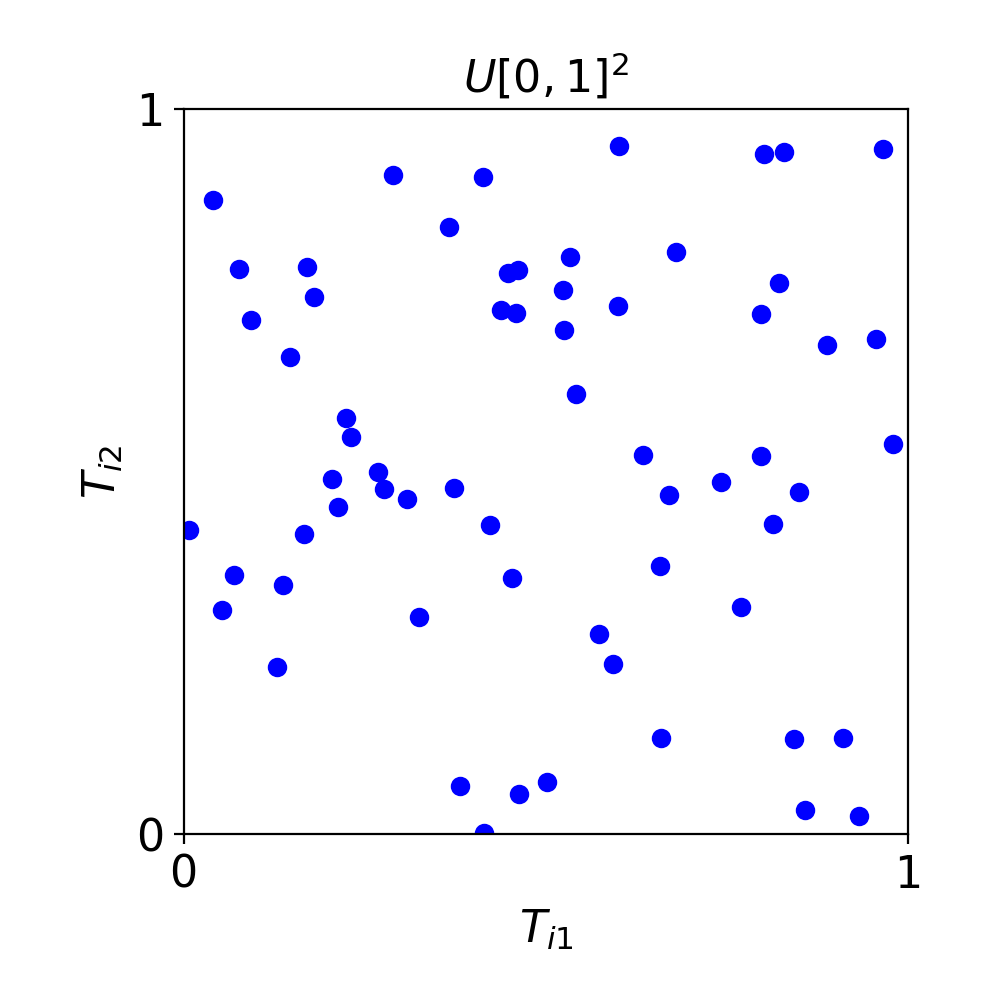
\includegraphics[height = 5cm]{ProgramsImages/iid_uniform_pts.png} \quad
	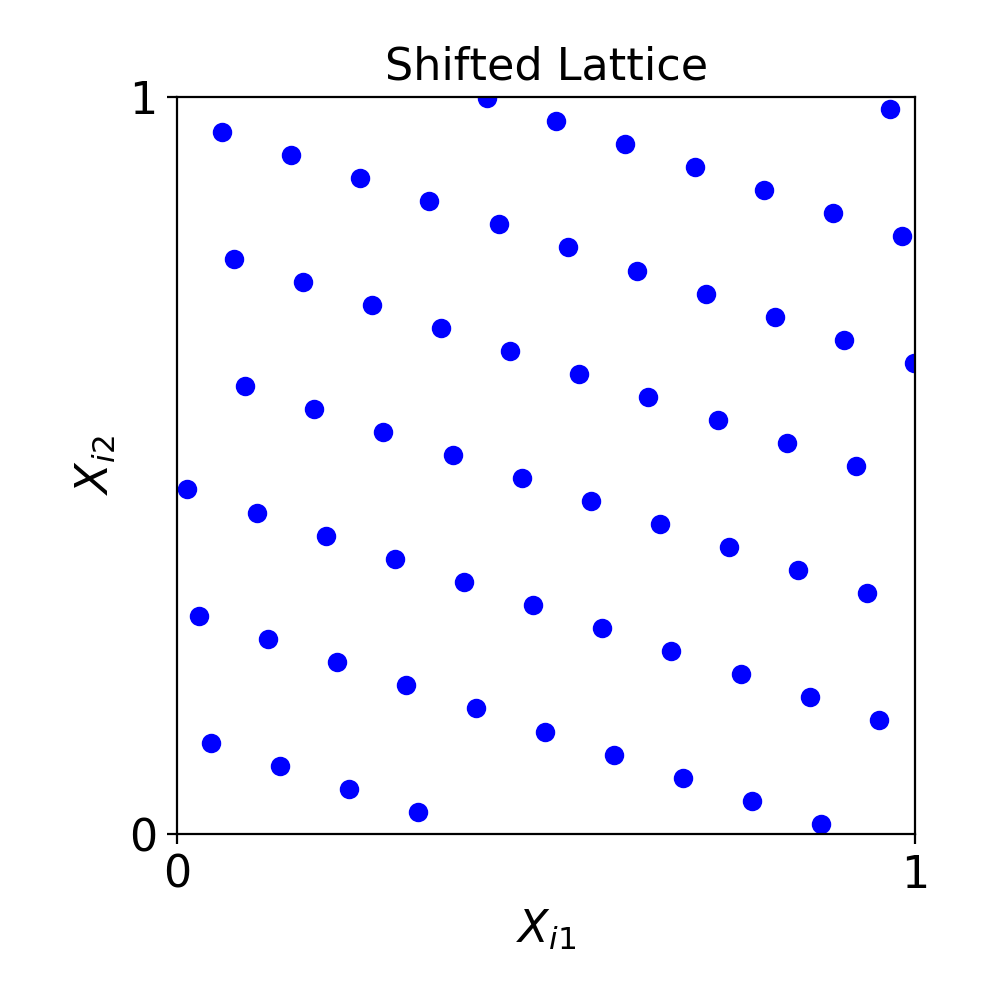
\includegraphics[height = 5cm]{ProgramsImages/lattice_pts.png} \quad
	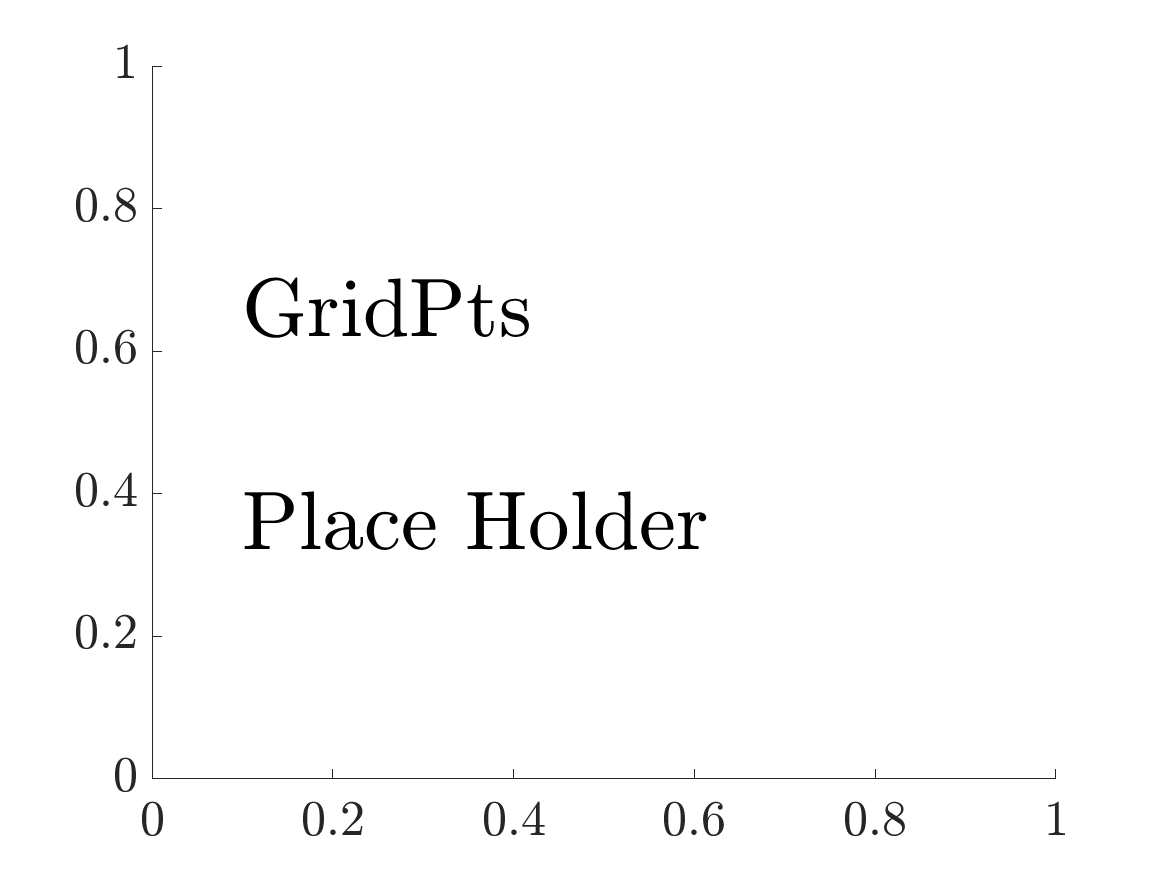
\includegraphics[height = 4cm]{ProgramsImages/GridPts.png}
	\caption{IID points (left), LD lattice points (center), and grid points (right).  The LD points have fewer gaps and clusters of points. \label{fig:iid_vs_ld}}
\end{figure}

The  points in the center of Figure \ref{fig:iid_vs_ld}, $\bX_1, \bX_2,  \ldots \LDSim \calu[0,1]^2$, are carefully coordinated with one another.  They might be deterministic or random.  They are designed to mimic the distribution $F$  in the sense that the empirical distribution function of  $\bX_1, \ldots \bX_n$---denoted $F_{\{\bX_i\}_{i=1}^n}$---is close to $F$.  (The empirical distribution for $n$  points assigns probability $1/n$ to each of point.)  A \emph{discrepancy}, $D(\{\bX_i\}_{i=1}^n, F)$, measures the size of $F - F_{\{\bX_i\}_{i=1}^n}$, and LD points make the discrepancy small.  Discrepancies are explained further in the next subsection.

The points on the right in Figure \ref{fig:iid_vs_ld} are grid points. While they may look even, they lack evenness in low dimensional projections.  Specifically, the grid points have only $\sqrt{n} = 8$ equally spaced values in each coordinate direction, whereas the LD points have $n=64$ equally spaced values.  For $d$-dimensional grids, there are only $n^{1/d}$ values in each coordinate direction, which is a weakness especially for large $d$.

\subsection{Efficiency Benefits from LD Sampling}
The root mean squared error of the sample mean, $\hmu_n$ in approximating the population mean, $\mu$, when IID samples are used is 
\begin{equation}
    \sqrt{\bbE\bigl[\abs{\mu - \hmu_n}^2\bigr]} = \frac{\std(Y)}{\sqrt{n}},  \quad \std(Y) = \sqrt{\int_{\cx} \abs{f(\bx) - \mu}^2 \, \dif F(\bx)}, \qquad \bX_1, \bX_2, \ldots \text{IID}.
\end{equation}
The smoothness requirement is minimal, and the error bound may be free from the curse of dimensionality (assuming that $\std(Y)$ does not explode with dimension), but the convergence rate is modest.  

For LD sampling the absolute error has an upper bound of
\begin{equation}
    \abs{\mu - \hmu_n}^2 \le D(\{\bX_i\}_{i=1}^n, F) \norm[\calf]{f},  \qquad \bX_1, \bX_2, \ldots \text{LD}.
\end{equation}
Here the Banach space $\calf$ typically requires somewhat more smoothness than the $L^2$ requirement for IID sampling, e.g., integrable mixed partial derivatives up to order one in each direction. The discrepancy,  $D(\{\bX_i\}_{i=1}^n, F)$, corresponds to the norm of the cubature error functional \cite{Hic97a}, and is typically $\Order(n^{-1 + \delta})$ for well-chosen LD sequences, where $\delta$ may be an arbitrarily small, positive number.

Figure \ref{fig:KeisterTimes} displays the results of approximating an integral from a computational physics example of Keister \cite{Kei96},
\begin{equation}
    \mu = \int_{\reals^d} \cos( \norm[2]{\bt}) \exp(-\norm[2]{\bt}^2) \, \dif \bt,
\end{equation}
for the case $d =?$ under several absolute error tolerances, $\varepsilon$, using QMCPy.  Both the number of function values and the computation time increase like $\Order(\varepsilon^{-2})$ for IID sampling and $\Order(\varepsilon^{-1-\delta})$ for LD sampling as $\varepsilon$ decreases. 


\begin{figure}
    \centering
    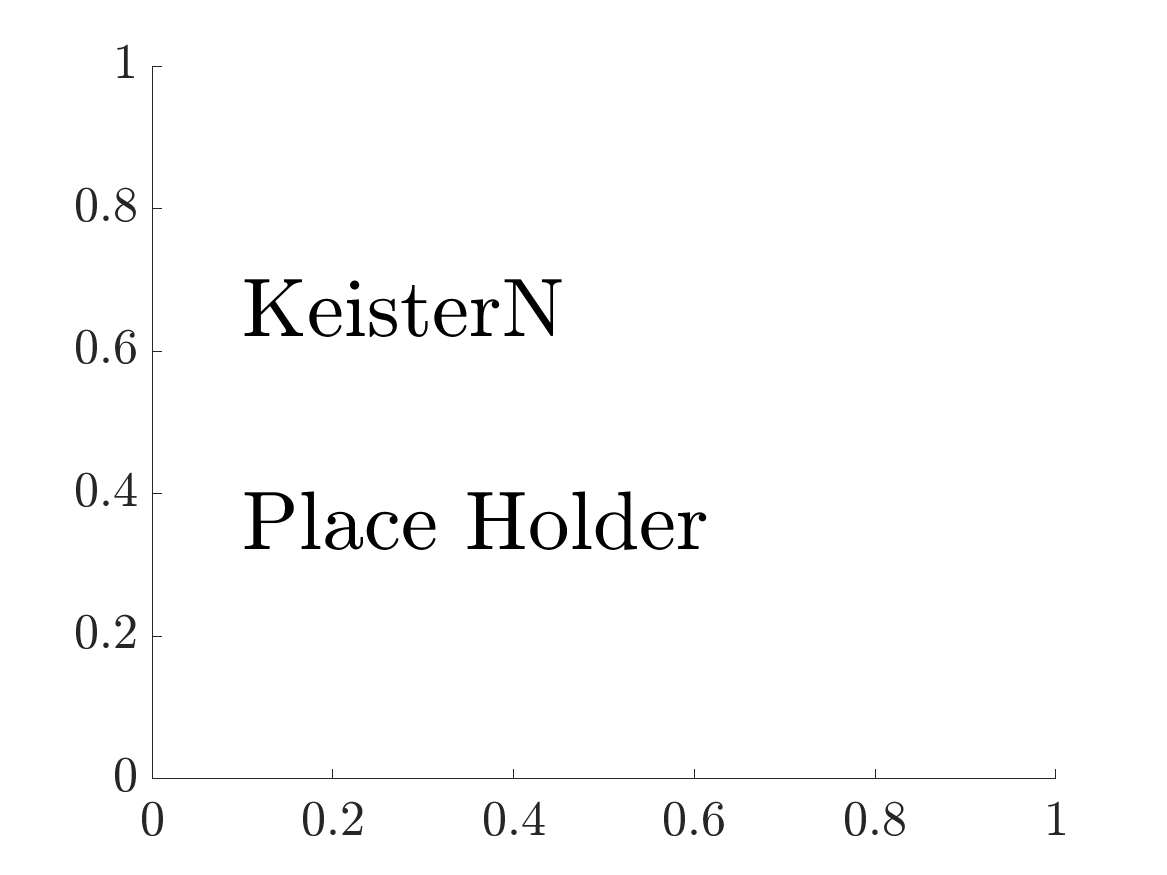
\includegraphics[height = 5.5 cm]{ProgramsImages/KeisterN.png} \qquad
    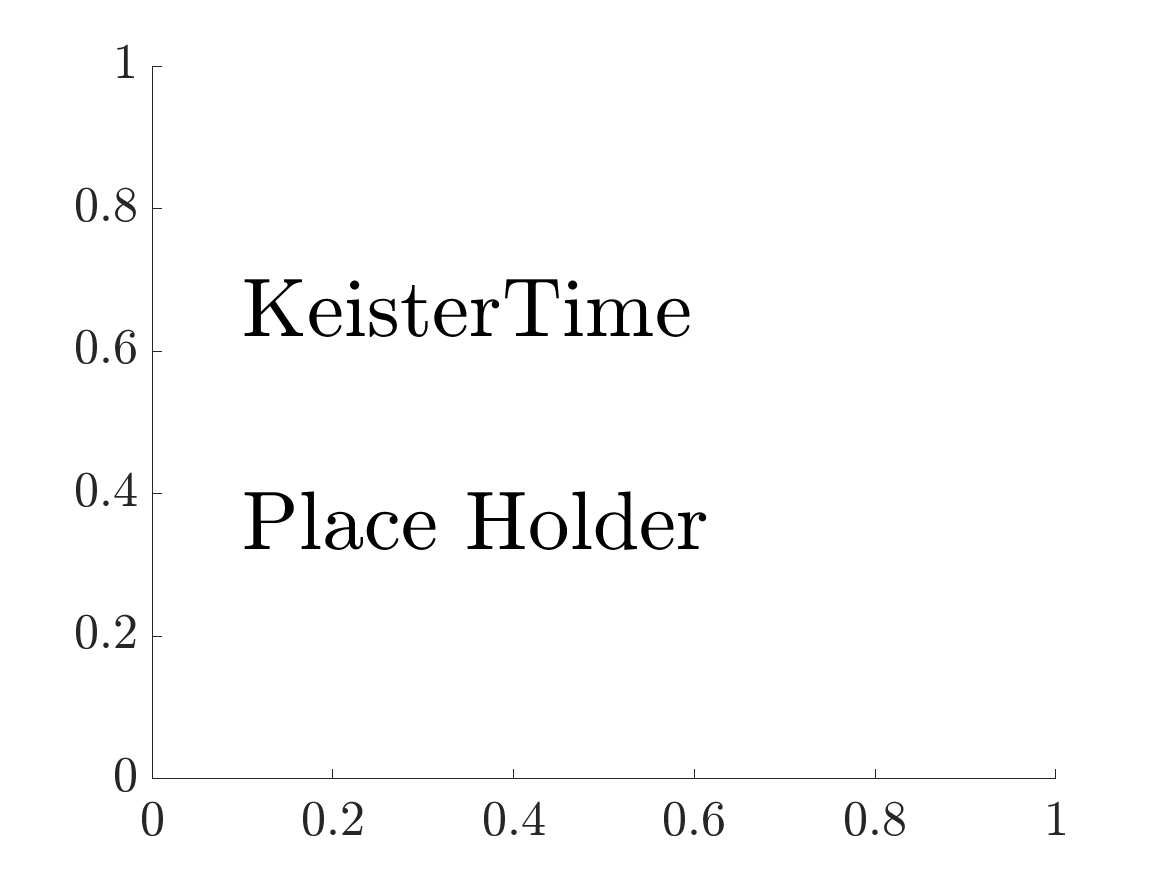
\includegraphics[height = 5.5 cm]{ProgramsImages/KeisterTime.png}
    \caption{Number of function values (left) and run time (right) required to compute the Keister integral \eqref{eq:Keister} using QMCPy.  LD sampling is much more efficient than IID sampling, especially as the error tolerance decreases.}
    \label{fig:KeisterTimes}
\end{figure}

The advantage of LD sampling is illustrated by the fact sharp divergence of the times and function values required as $\varepsilon$ decreases.  For $\varepsilon = $ the difference is already minutes for LD versus hours for IID and tens of thousands of function values for LD versus tens of millions of function values for IID.

The computational cost rates as $\varepsilon$ decreases for IID and LD sampling are essentially independent of $d$.  This is not the case for tensor product rules.  If the derivatives of $f$ up to total order $rd$ exist, then there exist tensor product rules that provide $\abs{\mu - \hmu_n} \le \varepsilon$  at a cost (time or function values) of $\Order(\varepsilon^{-d/r})$.  While increased smoothness, $r$, helps, it cannot overcome the curse of dimensionality (exponential growth of the cost with $d$).

\section{QMCPy Now}



\section{What QMCPy Should Become}


\section{Intellectual Merit}

QMCPy as an aggregator

parallel computing

GPUs

MLQMC

CUD

custom LD points

Plug and pay nets

importance sampling

more use cases

alternatives to discrepancy

Sobol' indices

higher order nets

%quantiles

kernel density estimation

sampling from large data


\section{Results from Previous Work}

Fred's

(Simon's?)

\section{Broader Impacts}

Proper handling of LD sequences 

Educating a wider user base

Branching into new applications

those who

QMCPy is proving ground


\newpage
\clearpage
%\pagenumbering{arabic}
\setcounter{page}{1}
%\renewcommand{\thepage}{D-\arabic{page}}

\bibliographystyle{spbasic}


{\renewcommand\addcontentsline[3]{} 
\renewcommand{\refname}{{\Large\textbf{References Cited}}}                   %%
\renewcommand{\bibliofont}{\normalsize}

\bibliography{FJH23,FJHown23}}
\end{document}
